\documentclass{beamer}
\usepackage{inconsolata}
\usepackage{caption}
\usepackage{color}
\usepackage{listings}
\usepackage{subfig}
\usepackage{cooltooltips}
\usepackage{hyperref}
\usepackage[normalem]{ulem}
\setbeamertemplate{navigation symbols}{}%remove navigation symbols
\usepackage{listings}
\usepackage{color}
\usepackage{framed}

\definecolor{background}{RGB}{39, 40, 34}
\definecolor{string}{RGB}{230, 219, 116}
\definecolor{comment}{RGB}{117, 113, 94}
\definecolor{normal}{RGB}{248, 248, 242}
\definecolor{identifier}{RGB}{166, 226, 46}



\lstset{
  language=C,               			% choose the language of the code
  alsolanguage=Python,            			% choose the language of the code
  alsolanguage=Java,            			% choose the language of the code
  numbers=none,                   		% where to put the line-numbers
  stepnumber=1,                   		% the step between two line-numbers.        
  numbersep=5pt,                  		% how far the line-numbers are from the code
  extendedchars=true,
  numberstyle=\tiny\color{black}\ttfamily,
  backgroundcolor=\color{background},  		% choose the background color. You must add \usepackage{color}
  showspaces=false,               		% show spaces adding particular underscores
  showstringspaces=false,         		% underline spaces within strings
  showtabs=false,                 		% show tabs within strings adding particular underscores
  frame=single,
  framerule=0pt,
  tabsize=4,                      		% sets default tabsize to 2 spaces
  captionpos=n,                   		% sets the caption-position to bottom
  breaklines=true,                		% sets automatic line breaking
  breakatwhitespace=true,         		% sets if automatic breaks should only happen at whitespace
  title=\lstname,                 		% show the filename of files included with \lstinputlisting;
  basicstyle=\color{normal}\tiny\ttfamily,					% sets font style for the code
  keywordstyle=\color{magenta}\tiny\ttfamily,	% sets color for keywords
  stringstyle=\color{string}\tiny\ttfamily,		% sets color for strings
  commentstyle=\color{comment}\tiny\ttfamily,	% sets color for comments
  emph={True, False, format_string, eff_ana_bf, permute, eff_ana_btr, KeyError,
  ValueError, ZeroDivisionError},
  emphstyle=\color{identifier}\tiny\ttfamily,
  morekeywords={with, as}
}

\lstset{literate=%
   *{0}{{{\color{cyan}0}}}1
    {1}{{{\color{cyan}1}}}1
    {2}{{{\color{cyan}2}}}1
    {3}{{{\color{cyan}3}}}1
    {4}{{{\color{cyan}4}}}1
    {5}{{{\color{cyan}5}}}1
    {6}{{{\color{cyan}6}}}1
    {7}{{{\color{cyan}7}}}1
    {8}{{{\color{cyan}8}}}1
    {9}{{{\color{cyan}9}}}1
}



\newenvironment{enum}{
\begin{enumerate}
  \setlength{\itemsep}{1pt}
  \setlength{\parskip}{0pt}
  \setlength{\parsep}{0pt}
}{\end{enumerate}}

\hypersetup{
  colorlinks=true,
  urlcolor=pink,
}

\title{Python 101}
\subtitle{Lec04 \\ Intermission}
\author{thoum}

\begin{document}
\frame{\titlepage}

\begin{frame}
\frametitle{What have we learned so far?}
  \begin{center}
  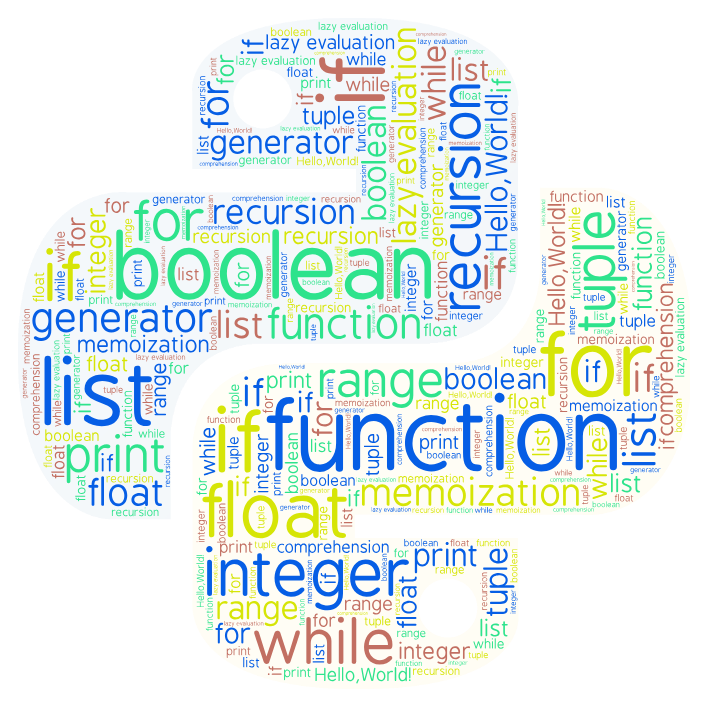
\includegraphics[width=80mm]{./python_art.png}
  \end{center}
\end{frame}

\begin{frame}
\frametitle{Turing Complete}
  We \textit{can} do everything\tiny{a computer can} \normalsize with what we have learned so far.
  
  But can \textit{you}?
\end{frame}

\begin{frame}
\frametitle{PSTP}
\begin{figure}
  \begin{center}
  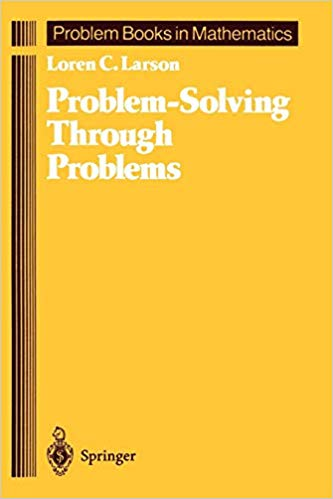
\includegraphics[width=50mm]{./cover.jpg}
  \caption*{https://www.amazon.com}
  \end{center}
\end{figure}
\end{frame}

\begin{frame}{Mini-Midterm}
  Open Book. Open Internet.
  Open Google. Open Stackoverflow.
\end{frame}

\begin{frame}{With an incentive}
  Those who finish upto Q4 until the end of the tutoring will get a
  \textbf{\textit{FREE}} cup of
  coffee at Starbucks\textsuperscript{\tiny\textregistered}.
\end{frame}

\begin{frame}
\frametitle{Q1. Goldbach Conjecture}
Every even integer greater than 2 is the sum of two prime numbers.

Let's prove it upto 10,000,000,000.
\end{frame}

\begin{frame}
\frametitle{Goldbach Conjecture}
\begin{figure}[H]
  \centering
  \begin{minipage}{.45\textwidth}
  \centering
    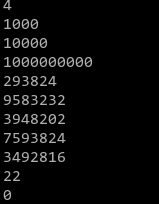
\includegraphics[width=45mm,height=40mm]{./gbach_input.png}
    \caption*{input}
  \end{minipage}
  \begin{minipage}{.45\textwidth}
  \centering
    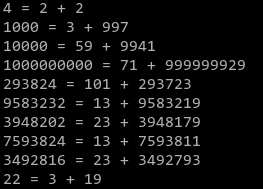
\includegraphics[width=45mm,height=40mm]{./gbach_output.png}
    \caption*{output}
  \end{minipage}
\end{figure}
\end{frame}

\begin{frame}{Step 0}
  Save as gbach.py
\end{frame}

\begin{frame}{Step 1}
  \begin{enumerate}
    \item The numbers come in seperate lines
    \item Do we have to store each numbers?
    \item We should terminate at 0.
  \end{enumerate}
\end{frame}

\begin{frame}{Step 1}
  Can we get the correct input?
  \begin{enumerate}
    \item The numbers come in seperate lines
    \item We should terminate at 0
    \item Do we have to store each numbers?
  \end{enumerate}
\end{frame}

\begin{frame}{Step 2}
  Now what?
  \begin{enumerate}
    \item Split the given number into two numbers
    \item See if the two numbers are \textit{primes}
  \end{enumerate}
\end{frame}

\begin{frame}{Step 2.1}
  Checking if a number is a prime.\\
  Ideas?
\end{frame}

\begin{frame}{Step 2.5}
  Checking if a number is a prime.
  \begin{enumerate}
    \item Generate the sieve of eratosthenes and check membership?
    \item Check N's divisors.
  \end{enumerate}
\end{frame}

\begin{frame}{Step 2.5}
  Checking if a number is a prime.
  \begin{enumerate}
    \item The sieve: (X). We have to store 455,052,511 numbers.
    \item Divisors: This seems better memory-wise.
  \end{enumerate}
\end{frame}

\begin{frame}[fragile]{Step 2.6}
  We need to make it into a function as is\_prime is used repeatedly.
  \begin{lstlisting}
  def is_prime(n):
      #Fill me in
  \end{lstlisting}
\end{frame}

\begin{frame}[fragile]{Step 2.7}
  Anatomy of is\_prime(n).\\
  For k: 2 ... n-1 \footnote{There is a better value, which is?}\\
    if n is divided by k:\\
        not a prime number\\
  if no divisor:\\
    is a prime number
\end{frame}

\begin{frame}[fragile]{Step 2.9}
  Check that is\_prime works well.
  It is often a good idea to test your program with
  random numbers, big numbers, and small numbers.
  \begin{enumerate}
    \item is\_prime(0)
    \item is\_prime(1)
    \item is\_prime(2)
    \item is\_prime(23334)
    \item is\_prime(1217)
    \item is\_prime(343313)
    \item is\_prime(10000000000)
  \end{enumerate}
\end{frame}

\begin{frame}[fragile]{Step 3.0}
  Splitting the numbers into two.
  (1, k-1) / (2, k-2)/ (3, k-3)...
\end{frame}

\begin{frame}[fragile]{Step 3.3}
  Now check if the split numbers are both primes\\
  is\_prime(k) and is\_prime(n-k)
\end{frame}

\begin{frame}[fragile]{Step 4.0}
  Time to pretty print it.
  How? Look it up
\end{frame}

\begin{frame}{Q2. Partitioning}
  Calculate the number of cases of partitioning number N with 1,2,3.\\
  4 =
  \begin{enumerate}
    \item 1+1+1+1
    \item 1+1+2
    \item 1+2+1
    \item 2+1+1
    \item 2+2
    \item 1+3
    \item 3+1
  \end{enumerate}
\end{frame}

\begin{frame}{Partitioning}
First Number: N
repeat N times.
\begin{figure}[H]
  \centering
  \begin{minipage}{.45\textwidth}
  \centering
    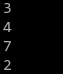
\includegraphics[width=45mm,height=40mm]{./part_input.png}
    \caption*{input}
  \end{minipage}
  \begin{minipage}{.45\textwidth}
  \centering
    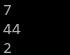
\includegraphics[width=45mm,height=40mm]{./part_out.png}
    \caption*{output}
  \end{minipage}
\end{figure}
\end{frame}

\begin{frame}{Step 0}
  Save as partition.py
\end{frame}

\begin{frame}{Step 1}
  Any ideas?\\
  Try writing some cases out.
\end{frame}

\begin{frame}{Step 1.5}
  Can you find any relationships?
\end{frame}

\begin{frame}{Step 1.9}
  Let's assume f(n) somehow magically calculates the answer for you.\\
  Then What?
\end{frame}

\begin{frame}{Step 2.0}
  Write out the relationship in your code.
\end{frame}

\begin{frame}{Step 3.0}
  Test it for large numbers.... what should we do?
\end{frame}

\begin{frame}{Challenge}
  We can change the recursive version with lists.\\
  Assume lst[n] gives the answer for you.\\
  Then what?
\end{frame}

\begin{frame}{Q3. Dumb Multiplication}
  123*999 = 91827\\
  999*999 = 818181
\end{frame}

\begin{frame}{Step 0}
  I will be providing less guides.
\end{frame}

\begin{frame}{Q4. Look and say sequence}
  Print the $N^{th}$ look and say sequence,
  a.k.a ant sequence.\\
  1, 11, 12, 1121, 122111....
\end{frame}

\begin{frame}{Do it!}
\end{frame}
\end{document}
